%
% teil1.tex -- Beispiel-File für das Paper
%
% (c) 2020 Prof Dr Andreas Müller, Hochschule Rapperswil
%
% !TEX root = ../../buch.tex
% !TEX encoding = UTF-8
%
\section{Gausssche Krümmung
\label{mongeampere:section:teil1}}
\kopfrechts{Gausssche Krümmung}
Damit wir verstehen wie die Monge-Ampèresche Gleichung mit der 
Krümmung einer Fläche zusammenhängt, brauchen wir zuerst eine Methode diese 
Krümmug zu beschreiben.
Die Herleitungen in diesem Kapitel basieren auf \cite{mongeampere:smirnow}.
Wir betrachten dabei die Fläche
\begin{equation}
  x = \varphi(u,v), \quad y = \psi(u,v), \quad z = \omega(u,v)
  \label{mongeampere:areaparam}
\end{equation}
Die Fläche kann man in der Parameterform auch als Radiusvektor
\begin{equation}
  \vec r (u, v) =
  \begin{pmatrix}
    x(u,v) \\
    y(u,v) \\
    z(u,v) \\
  \end{pmatrix}
  \label{mongeampere:rad}
\end{equation}
schreiben.
Leitet man diesen Radiusvektor nach den Prametern $u$ und $v$ ab bekommnt man zwei Tangenten
$\vec r_u$ und $\vec r_v$,
mit welchen die Flächennormale 
\begin{equation}
  \vec m = \frac{\vec r_u \times \vec r_v}{\sqrt{(\vec r_u \times \vec r_v)^2}} 
  \label{mongeampere:norm}
\end{equation}
beschrieben werden kann, wobei $(\cdot)^2$ für das Skalarprodukt eines Vektores mit sich selber steht.

\subsection{Erste Fundamentalform
\label{mongeampere:subsection:finibus}}
\ref{mongeampere:section:teil2}.
Die erste Fundamentalform beschreibt die innere Geometrie einer Fläche.
Betrachtet man das Quadrate des Bogendifferential einer auf der Fläche 
beschriebenen Kurve $S(u,v)$ so ist 
\begin{equation}
  \begin{split}
    \dd s^2 &= \dd x^2 + \dd y^2 + \dd z^2 \\
          &= \left(\pdv{x}{u}\dd u + \pdv{x}{v}\dd v  \right)^2
          + \left(\pdv{z}{u}\dd u + \pdv{z}{v}\dd v  \right)^2
          + \left(\pdv{z}{u}\dd u + \pdv{z}{v}\dd v  \right)^2.
  \end{split}
  \label{mongeampere:bogdiff}
\end{equation}
Rechnet man die Klammern aus, erhält man 
\begin{equation}
    \dd s^2 = E(u,v) \dd u^2 + 2F(u,v) \dd u \, \dd v + G(u,v)\dd v^2
    \label{mongeampere:1fundform}
\end{equation}
mit
\begin{align}
     E(u,v) &= \left(\pdv{x}{u} \right)^2 +
     \left(\pdv{y}{u} \right)^2 +
     \left(\pdv{z}{u} \right)^2 
            &= \vec r_u^2\\
     F(u,v) &= 
     \pdv{x}{u} \cdot \pdv{x}{v} +
     \pdv{y}{u} \cdot \pdv{y}{v} +
     \pdv{z}{u} \cdot \pdv{z}{v}
            &= \vec r_u \cdot \vec r_v \\
      G(u,v) &= \left(\pdv{x}{v} \right)^2 +
     \left(\pdv{y}{v} \right)^2 +
     \left(\pdv{z}{v} \right)^2 
             &= \vec r_v ^2\\
  \label{mongeampere:1fundbed}
\end{align}
Diese Forulierung vom Bogendifferential ist als erste Fundamentalform bekannt.
Man kann sie auch in Form des Metrischen Tensors 
\begin{equation}
  g_{ij} = \begin{pmatrix}
    E & F \\
    F & G \\
  \end{pmatrix}
  \label{mongeampere:erstmettens}
\end{equation}
beschreiben.

Die Koeffizienten der ersten Fundamentalform können auch für das Flächenelement mit
\begin{equation}
  \dd S = |\vec r_u \times \vec r_v|\dd u \dd v = \sqrt{EG-F^2} \dd u \dd v.
  \label{mongeampere:ds}
\end{equation}
verwendet werden.

\subsection{Zweite Fundamentalform}
Die zweite Fundamentalform befasst sich mit der äusseren Geometrie einer 
Fläche und beschreibt wie sich die Tangente entlang einer Flächenkurve verändert.
Dafür betrachten wir wieder die Kurve $S(u,v)$ mit einem Tangeteneinheitsvektor 
$\vec t$;
Da die Kurve auf der Fläche liegt ist $\vec t$ in jedem Punkt senkrecht auf der 
Flächennormale $\vec m$, womit $\vec t \cdot \vec m = 0$ gilt. 
Berechnen wir nun 
\begin{equation}
  \dv{\vec t \cdot \vec m}{s}
  \label{mongeampere:2fund0}
\end{equation}
erhalten wir 
\begin{equation}
  \dv{\vec t}{s} \cdot \vec m + \vec t \cdot \dv{\vec m}{s} = 0. 
  \label{mongeampere:2fund1}
\end{equation}
Der Term $\dd \vec t / \dd s = \varrho^{-1} \vec n$ beschreibt einen Vektor in Richtung der Kurvennormalen 
$\vec n$ mit der Länge $\varrho^{-1}$, welche den inversen Krümmungsradius der Kurve 
darstellt.
Somit können wir \eqref{mongeampere:2fund1} umformen nach
\begin{equation}
  \frac{\vec n \cdot \vec m}{\varrho} = - \frac{\dd \vec r \cdot \dd \vec m }{\dd s^2} 
  \label{mongeampere:2fund2}
\end{equation}
Rechnet man den Zähler als Funktion der Parameter $u, v$ aus, erhält man die zweite 
Gausssche Fundamentalform
\begin{equation}
  \mathrm{I\!I} = \dd \vec r \cdot \dd \vec m  = L(u, v) \dd u^2 + 2 M (u,v) \dd u \dd v + N(u,v) \dd v^2.
  \label{mongeampere:2fund}
\end{equation}
mit den Koeffizienten
\begin{align*}
  L &= \vec r_{uu} \cdot \vec m \\ 
  M &= \vec r_{uv} \cdot \vec m \\
  N &= \vec r_{vv} \cdot \vec m.
  \label{mongeampere:2fundkoef}
\end{align*}
Die zweite Fundamentalform beschreibt wie start sich die Fläche an einem Punkt
von der Tangentialebene entfernt, wenn sich die Parameter etwas ändern.
Wie stark sich die Fläche von der Tangentialebene entfernt, hat einen Zusammenhang mit der Krümmung der Fläche.

In \eqref{mongeampere:2fund2} haben wir die zweite Fundamentalform in Richtung einer Flächenkruve mit
dem Quadrat ihres Bigendifferentiales normalisiert.
Damit erhielten wir den Anteil der Krümmung der Flächenkruve, die von der Krümmung der Fläche kommt.

\subsection{Krümmung}
Um den Begriff der Krümmung auf einer Fläche etwas besser zu verstehen
untersuchen wir die Krümmung von Normalenschnitte.
Ein Normanlenschnitt ist die Schnittkurve, zwischen der Fläche und der Ebene, welche durch einen Vektor auf 
der Tangentialebene der Fläche und der Flächennormalen aufgespannt wird.
Da die Normale eines Normalenschnittes bis auf das Vorzeichen gleich der Flächennormale ist, ist der 
Krümmungsradius
\begin{equation}
  \frac{1}{R} = \pm \frac{L \dd u^2 + 2 M \dd u \dd v + N \dd v^2}
                  {E \dd u^2 + 2F \dd u \, \dd v + G\dd v^2}.
  \label{mongeampere:normkrum}
\end{equation}
Diese Formulierung erlaubt uns ein paar Eigenschaften der Fläche zu bestimmen.
Da der Nenner $\dd s^2$ entspricht, ist er immer positiv. 
Teilen wir den Zähler durch $\dd u^2$ erhalten wir den Quadratischen Term
\begin{equation}
   L + 2M \frac{\dd v}{\dd u} + N \frac{\dd v^2}{\dd u ^2}.
  \label{mongemapere:dsik}
\end{equation}
Untersucht man die Diskriminante dieses Terms ergeben sich drei Fälle
\begin{enumerate}
  \item $M^2 - LN < 0$: Das Vorzeichen des Krümmungsradius ändert sich nicht, somit geht die Krümmung für alle 
    Flächennormalen in dieselbe Richtung. 
    Ein solcher Punkt wird \emph{elliptisch} genannt. Ein Beispiel ist, wie der 
    Name schon vermuten lässt, eine Ellipse.
  \item $M^2 - LN > 0$: Das Vorzeichen des Krümmungsradius ändert sich, somit wechselt die Richtung der Krümmung.
    Ein solcher Punkt wird \emph{hyperbolisch} genannt. Ein Beispiel ist ein Sattelpunkt.
  \item $M^2 - LN = 0$: Das Vorzeichen des Krümmungsradius ändert sich nicht, jedoch wird der Radius für einen 
    bestimmten Normalenschnitt null. 
    Ein solcher Punkt wird \emph{parabolisch} genannt. Eine prarbolische Fläche ist die Mantelfäche eines Zylinders. 
\end{enumerate}
In Abbildung \ref{mongeampere:arten} sind Beispiele zu den Flächentypen zu sehen.
\begin{figure}
	\centering
	\subfigure[]{
		\label{mongeampere:ellip}
		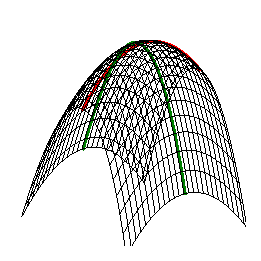
\includegraphics[width=0.31\textwidth]{papers/mongeampere/fig/ellip}}
	\subfigure[]{
		\label{mongeampere:sattel}
		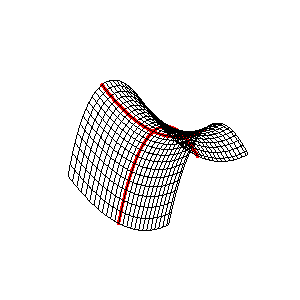
\includegraphics[width=0.31\textwidth]{papers/mongeampere/fig/saddle}} 
	\subfigure[]{
		\label{mongeampere:para}
		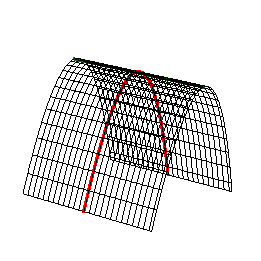
\includegraphics[width=0.31\textwidth]{papers/mongeampere/fig/para}}
	\caption{(a) Elliptischer Punkt (b) Hyperbolischer Punkt  (c) Parabolischer Punkt. In rot sind die jeweiligen Hautpkrümmungen zu sehen.}
	\label{mongeampere:arten}\end{figure}
\subsubsection{Hauptkrümmungsradien}
Die Hauptkrümmungsradien an einem Punkt einer Fläche sind definiert als der kleinste und grösste Krümmungsradius an diesem Punkt.
Anhand des Ausdrucks \eqref{mongeampere:normkrum} lassen sich die beiden Hauptkrümmungsradien berechnen.
Dafür leiten wir den Term nach den Tangentenrichtungen $\frac{\dd v}{\dd u}$ und $\frac{\dd u}{\dd v}$ ab.
Mit etwas Umformen erhalten wir die quadratische Gleichung
\begin{equation}
  (EG - F^2)\frac{1}{R^2} + (2FM - EN - GL)\frac{1}{R} + (LN-M^2) = 0.
  \label{mongeampere:mainkrum}
\end{equation}
Die Lösungen dieser Gleichung sind die beiden invertierten Hauptkrümmungsradien $R_1^{-1}$ und $R_2^{-1}$.
Wie wir aber im folgenden Abschnitt sehen werden, brauchen wir für die Gausssche Krümmung die Gleichung nicht 
zu lösen.

\subsection{Gausssche Krümmung}
Die Krümmung wie wir sie in \eqref{mongeampere:2fund2} beschrieben haben hat das Problem, dass
ihr Vorzeichen abhängig von der Normalenrichtung ist.
Die Gausssche Krümmung ist ein Krümmungsmass, welches von solchen Faktoren unabhängig ist.
Sie is definiert als 
\begin{equation}
  K = \frac{1}{R_1 R_2} = \frac{LN-M^2}{EG-F^2}.
  \label{mongeampere:gausskrumm}
\end{equation}
Da sie die beiden Hauptkrümmungsradien mulitipliziert ist sie immer positiv wenn 
beide Krümmungradien das gleiche Vorzeichen haben, und negativ falls sie sich unterscheiden.
Ausserdem lässt sich anhand des Voryeichens bestimmen ob ein Punkt elliptisch, hzperbolisch oder parabolisch 
ist, da die Diskriminante der zweiten Normalform im Zähler ist.

Eine interessante Eigenschaft, welche Gauss als \emph{Theoreme egregium} publiziert hat, ist, dass
die Gausssche Krümmung mit den Koeffizienten der ersten Fundamentalform und ihren Ableitungen beschrieben werden kann.
Das Bedeutuet, dass die innere Geometrie einer Fläche bestimmt, welche Gausssche Krümmung sie hat.
Im Umkehrschluss folgt, dass sich eine Fläche nicht auf eine andere Fläche mit einer anderen Krümmung abbilden
lässt, ohne das Längen oder Winkel gestreckt werden.
Dieses Theorem erklärt also, wieso es keine längen und winkeltreue flache Abbildungen der Erdoberfläche gibt.

